% !TEX program = xelatex
\documentclass[11pt,a4paper]{article}
\usepackage{graphicx}
\usepackage{ctex}
\usepackage{float}
\usepackage{geometry}
\usepackage{url}
\usepackage{caption}
\usepackage{fontspec}
\setmainfont{DejaVu Serif}
\geometry{left=2.5cm,right=2.5cm,top=2.5cm,bottom=2.5cm}
\title{HW5 — Tutte Parameterization 实验报告}
\author{胡广理  PB24010500}
\date{\today}
\begin{document}
\maketitle
\begin{abstract}
本实验实现并比较了基于均匀权重（Uniform）与余切权重（Cotangent）的 Tutte 参数化，并在三维模型表面回写 UV 后贴图展示结果。本文记录了完整的操作步骤、节点连线、关键参数值、实验结果和文件输出位置（含 `Results.usd`）。
\end{abstract}

\section{环境与文件位置}
- 项目根目录：USTC\_CG（略）
- 实验图像：\url{Homeworks/5_tutte_parametrzation/pdf/pictures/}
- 输入模型：\url{Homeworks/5_tutte_parametrzation/data/meshes/Balls.usda}
- 贴图图像：\url{Homeworks/5_tutte_parametrzation/data/test.png}
- 本次最终保存的 USD：\url{Homeworks/5_tutte_parametrzation/pdf/Results.usd}（注意：你打开时使用的是本机的绝对路径，保存时请确认该文件路径对提交包有效）

\section{节点与数据流概览}
本实验在 Ruzino 的节点编辑器按照下列数据流执行：
\begin{enumerate}
  \item \verb|read_usd|（读取 USD 模型）
  \item \verb|hw5_boundary_map|（可选：将边界映射到凸平面区域 — 方形或圆形）
  \item \verb|hw5_param|（求解 Tutte 参数化，输出参数化几何并写入顶点 \verb|Texcoords|）
  \item \verb|mesh_decompose|（从原始立体读出顶点/拓扑）
  \item \verb|mesh_decompose|（从参数化结果读出 \verb|Texcoords|）
  \item \verb|mesh_compose|（将原始顶点/拓扑与参数化得到的 \verb|Texcoords| 组合回一个带 UV 的 Mesh）
  \item \verb|set_texture|（将 \texttt{test.png} 赋给该 Mesh 的材质）
  \item \verb|write_usd|（写入 stage）
\end{enumerate}

\section{详细操作步骤（逐步精确）}
下面列出在 Ruzino GUI 中逐步操作（点击、填值、拖拽均写明）：
\subsection{读取模型}
1. 右键 → 搜索 \verb|read_usd| → 添加节点。
2. 在参数面板：\verb|File Name| 填入：\url{/home/hgl/code/ustc/USTC_CG/Homeworks/5_tutte_parametrzation/data/meshes/Balls.usda}。\verb|Prim Path| 填入：\verb|/Balls/Balls|。\verb|Time Code|=0。

\subsection{参数化（生成 UV）}
1. （可选）添加 \verb|hw5_boundary_map|，将 \verb|read_usd| 输出拖到它的 \verb|Geometry| 输入；在 \verb|Shape| 填 \verb|square| 或 \verb|circle|（分别得到方形/圆形边界映射）。
2. 添加 \verb|hw5_param|，将 \verb|hw5_boundary_map| 的输出（或直接 \verb|read_usd| 输出）连到 \verb|hw5_param| 的 \verb|Geometry|。
3. 若使用余切权重，额外将 \verb|read_usd| 输出连到 \verb|hw5_param| 的 \verb|Reference Geometry| 输入。
4. 在 \verb|hw5_param| 的 \verb|Weight Type| 填入：\verb|uniform| 或 \verb|cotangent|（节点内部会归一化并转为小写）。

\subsection{提取与重构用于贴图的立体网格}
1. 添加第一个 \verb|mesh_decompose|，连接 \verb|read_usd| 输出到其 \verb|Mesh| 输入。该节点输出 \verb|Vertices|、\verb|FaceVertexCounts|、\verb|FaceVertexIndices|、\verb|Normals|。
2. 添加第二个 \verb|mesh_decompose|，连接 \verb|hw5_param| 输出到其 \verb|Mesh| 输入，取其 \verb|Texcoords| 输出（参数化得到的 UV）。
3. 添加 \verb|mesh_compose|，并将第一个 \verb|mesh_decompose| 的 \verb|Vertices|、\verb|FaceVertexCounts|、\verb|FaceVertexIndices|、\verb|Normals| 分别连接到 \verb|mesh_compose| 对应输入，将第二个 \verb|mesh_decompose| 的 \verb|Texcoords| 连接到 \verb|mesh_compose| 的 \verb|Texcoords|。

\subsection{贴图与导出}
1. 将 \verb|mesh_compose| 的输出连到 \verb|set_texture| 的 \verb|Geometry|，在 \verb|set_texture| 的 \verb|Texture Name| 输入：\url{/home/hgl/code/ustc/USTC_CG/Homeworks/5_tutte_parametrzation/data/test.png}（绝对路径以避免解析为相对于可执行程序的相对路径错误）。
2. 将 \verb|set_texture| 输出连到 \verb|write_usd| 的 \verb|Geometry| 输入，在 \verb|write_usd| 的 \verb|Sub Path| 填 \verb|/Result|（或其他 prim 名）。
3. 在 Ruzino 主菜单执行：File → Save Stage As...，填写保存路径（例如 \verb|Homeworks/5_tutte_parametrzation/pdf/Results.usd|），确认保存。

\section{实验结果（图示）}
下面插入你放在 \verb|pdf/pictures| 下的图片，按需要在报告中替换或裁剪。
\begin{figure}[H]
  \centering
  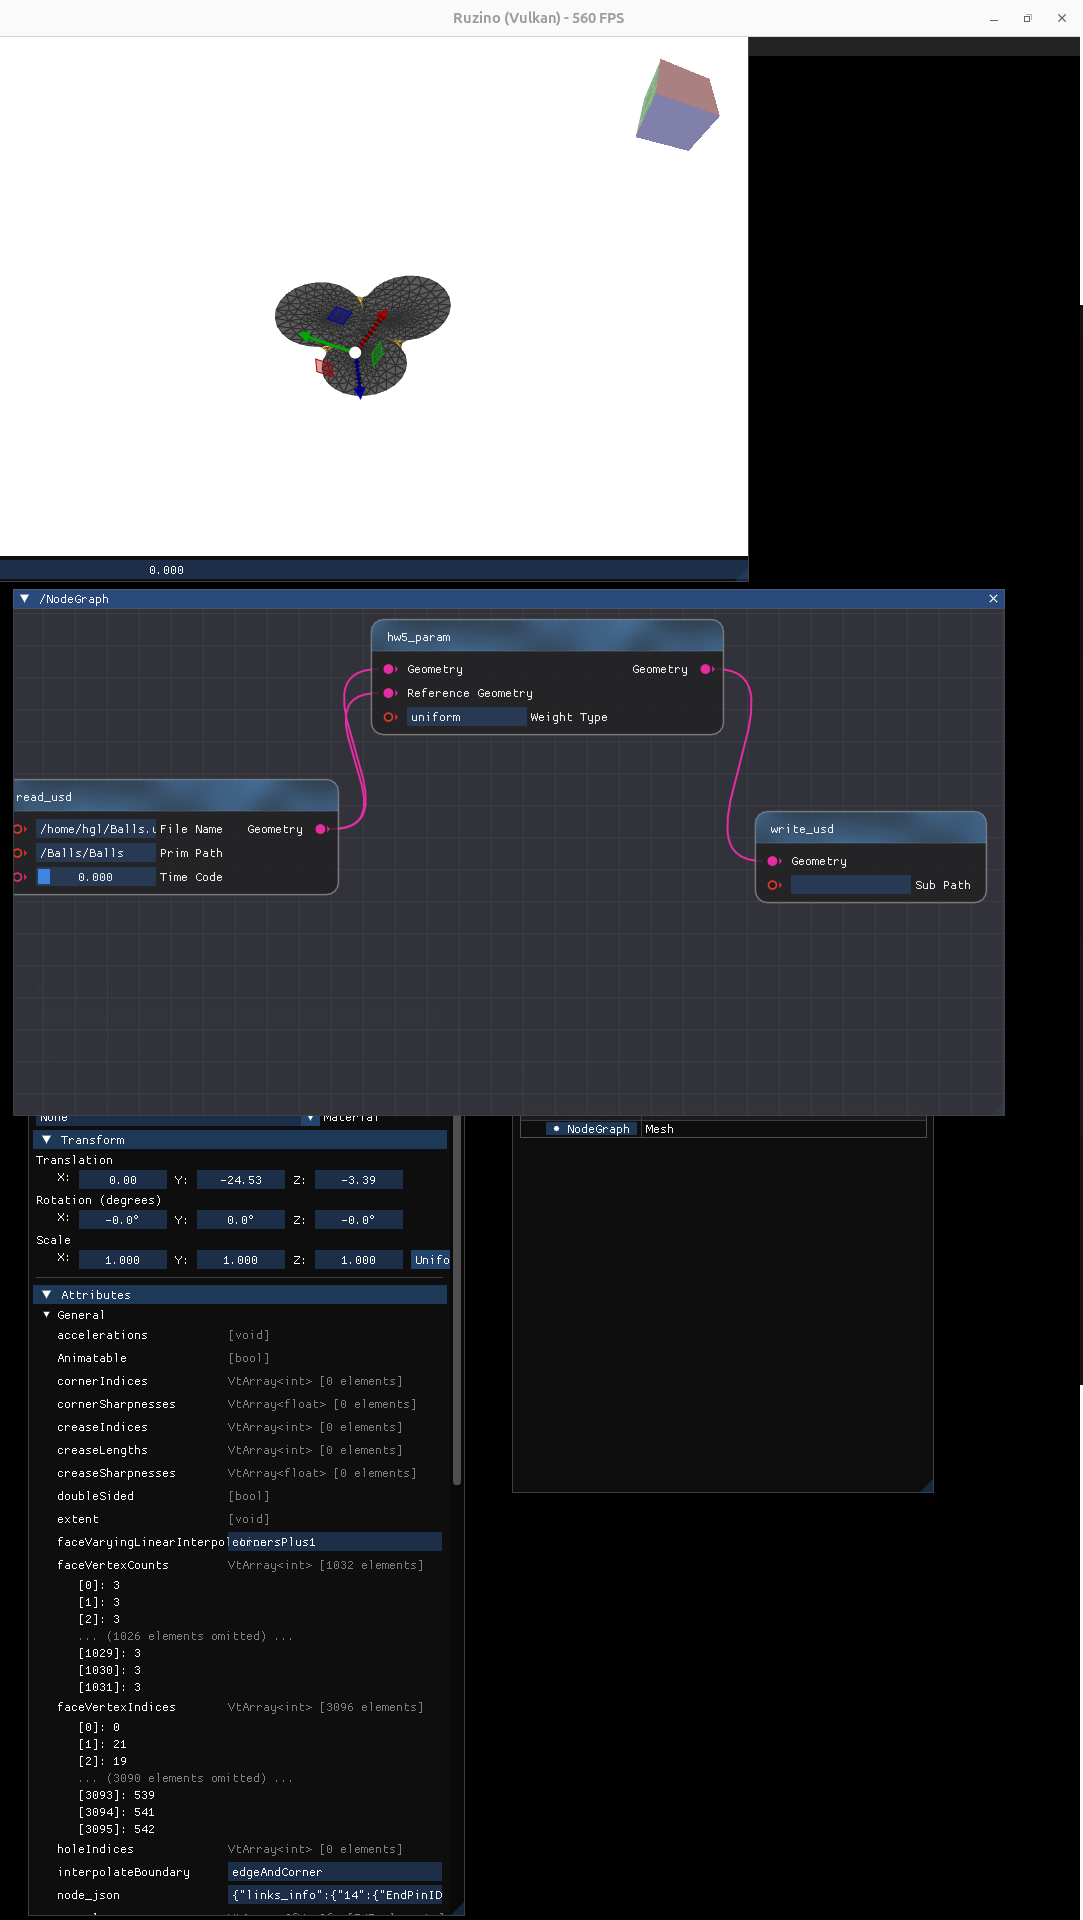
\includegraphics[width=0.9\textwidth]{pictures/初始映射_uniform.png}
  \caption{均匀权重（Uniform）初始参数化（平面）}
\end{figure}

\begin{figure}[H]
  \centering
  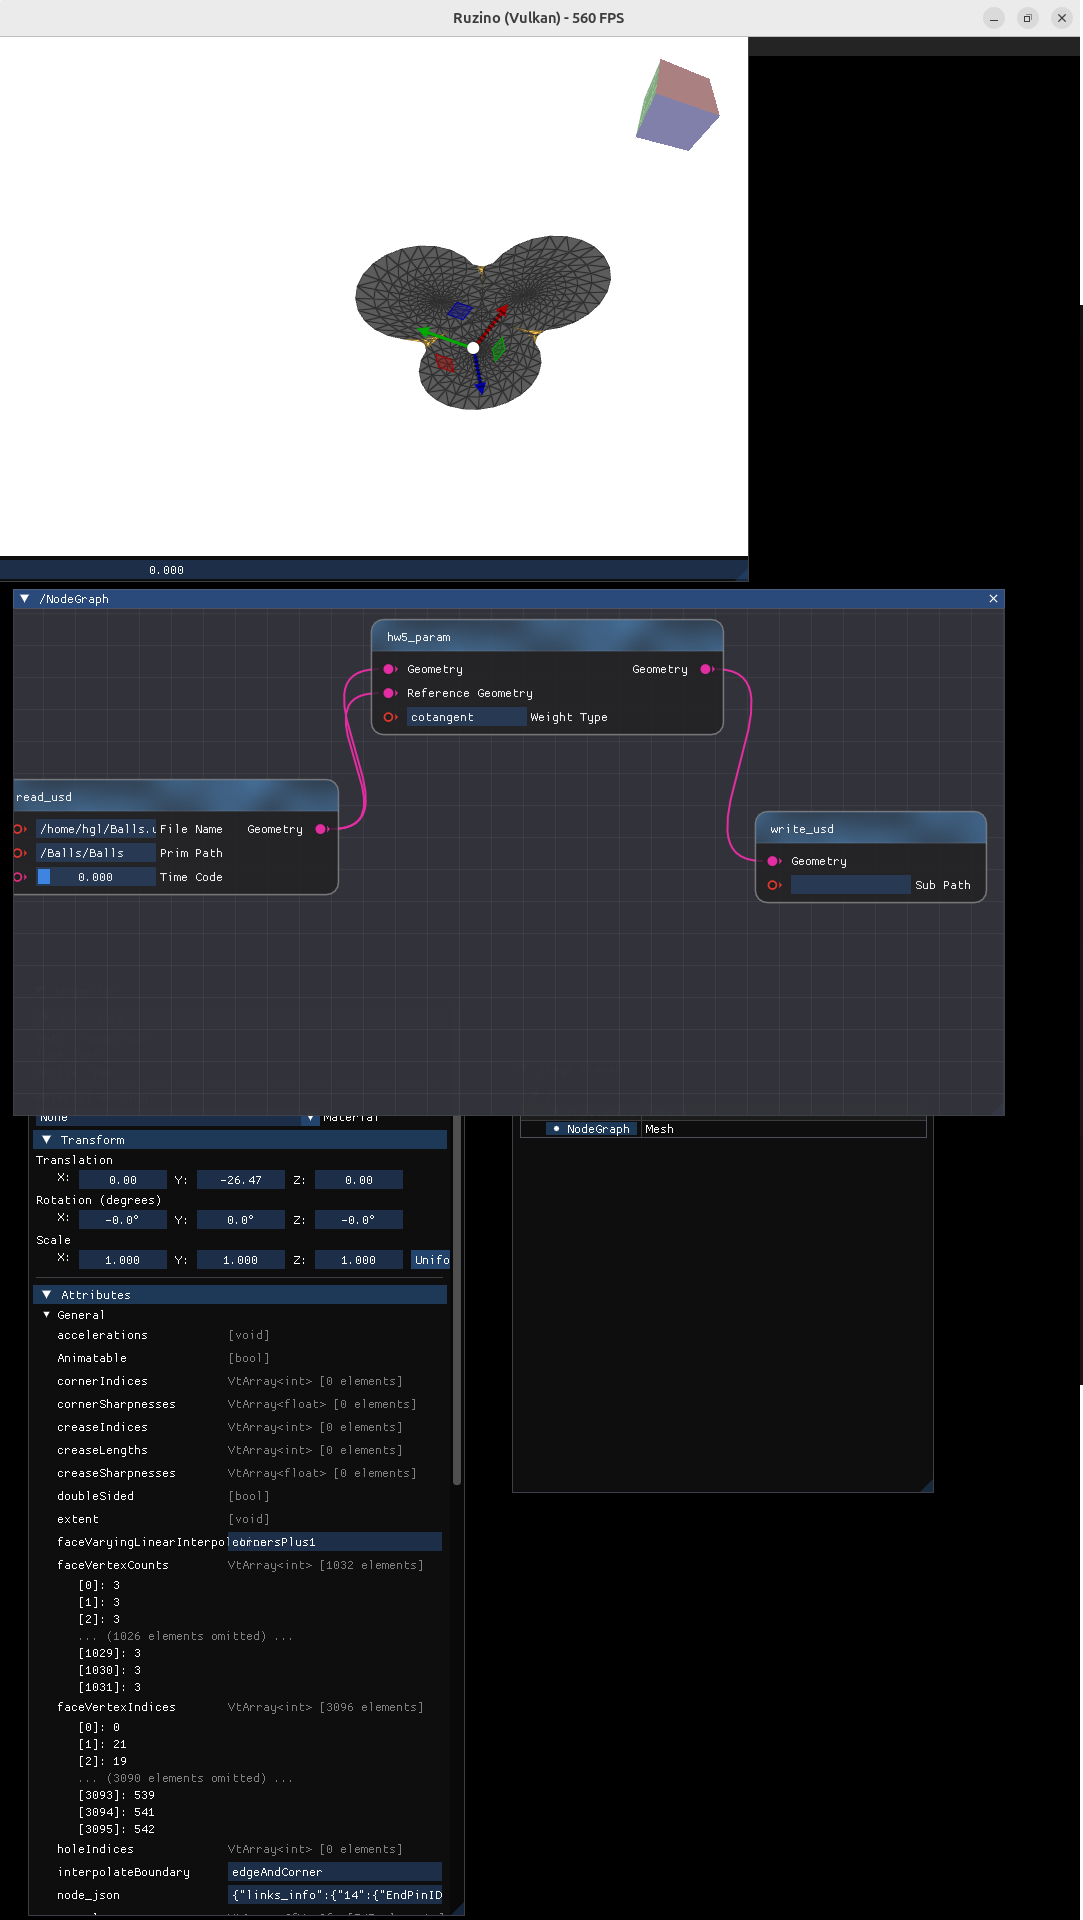
\includegraphics[width=0.9\textwidth]{pictures/初始映射_cotangent.png}
  \caption{余切权重（Cotangent）初始参数化（平面）}
\end{figure}

\begin{figure}[H]
  \centering
  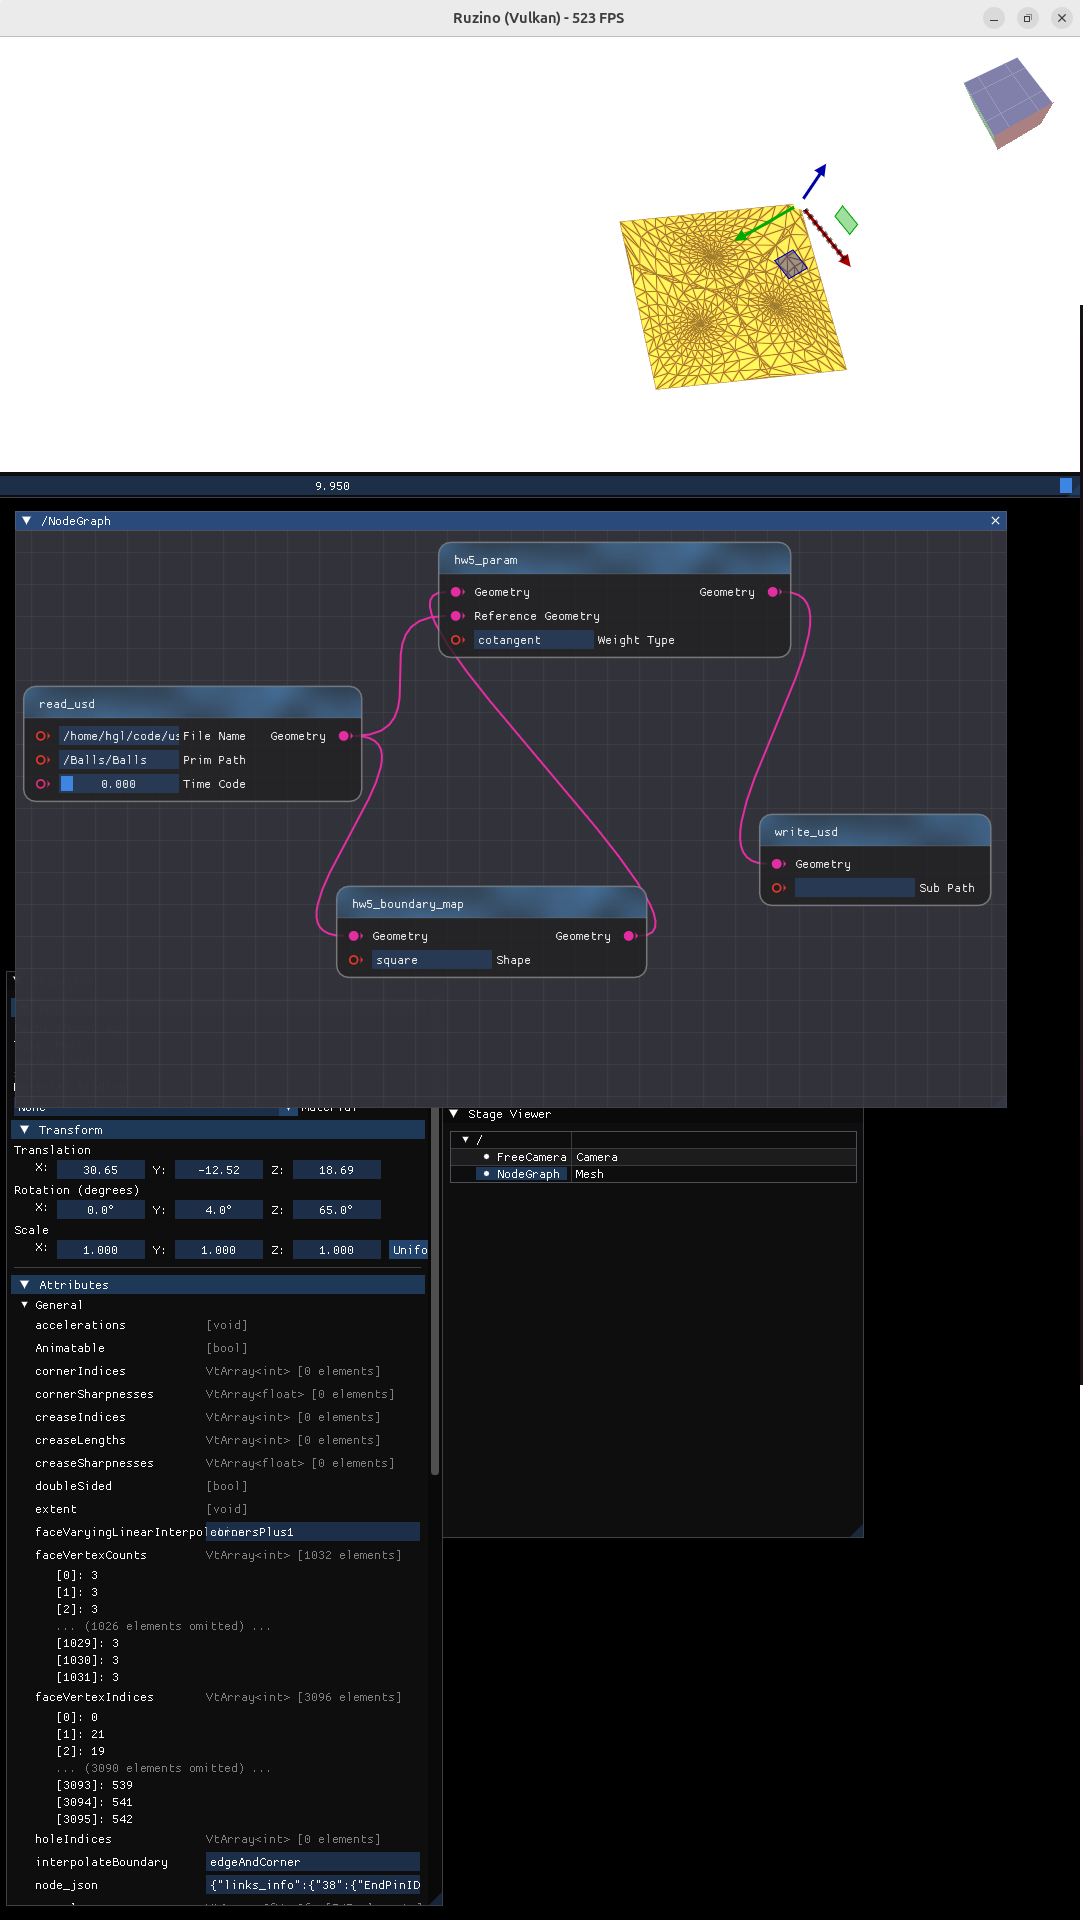
\includegraphics[width=0.9\textwidth]{pictures/边界映射_square.png}
  \caption{边界映射：方形}
\end{figure}

\begin{figure}[H]
  \centering
  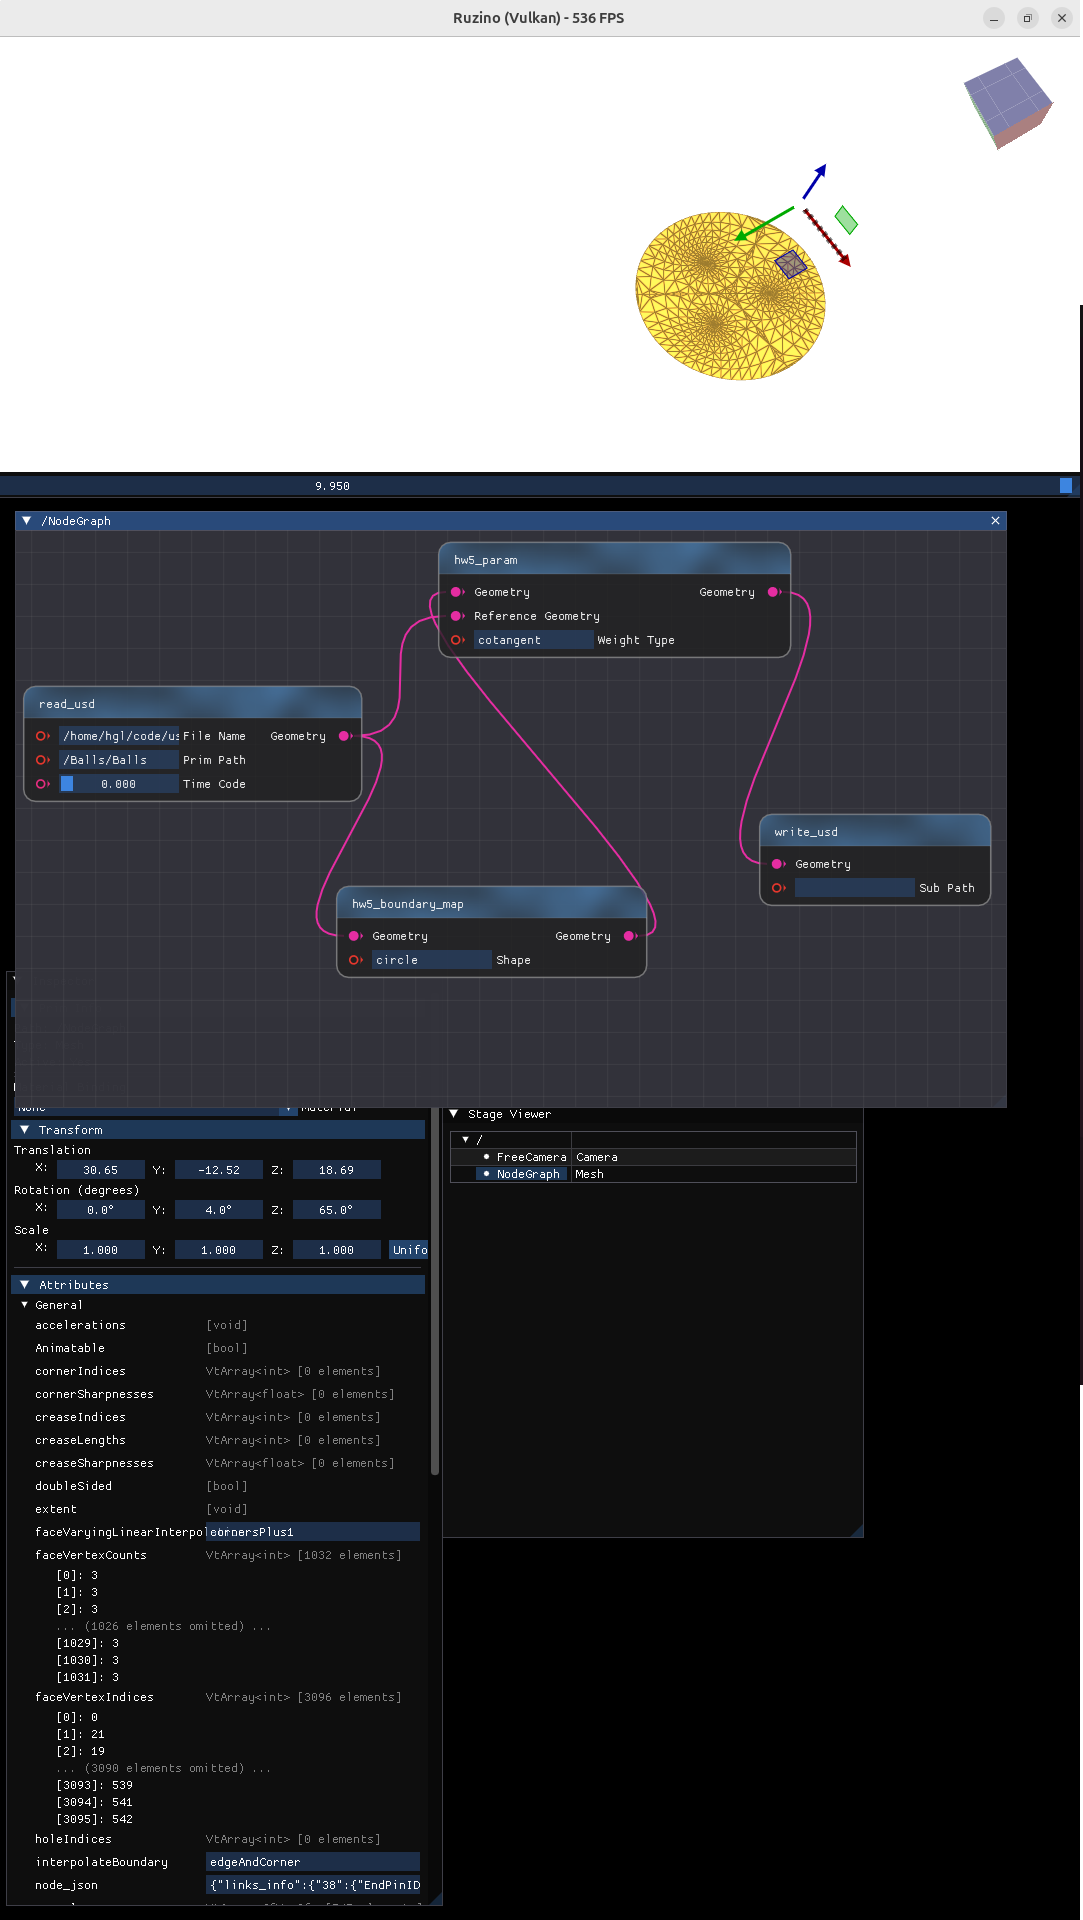
\includegraphics[width=0.9\textwidth]{pictures/边界映射_circle.png}
  \caption{边界映射：圆形}
\end{figure}

\begin{figure}[H]
  \centering
  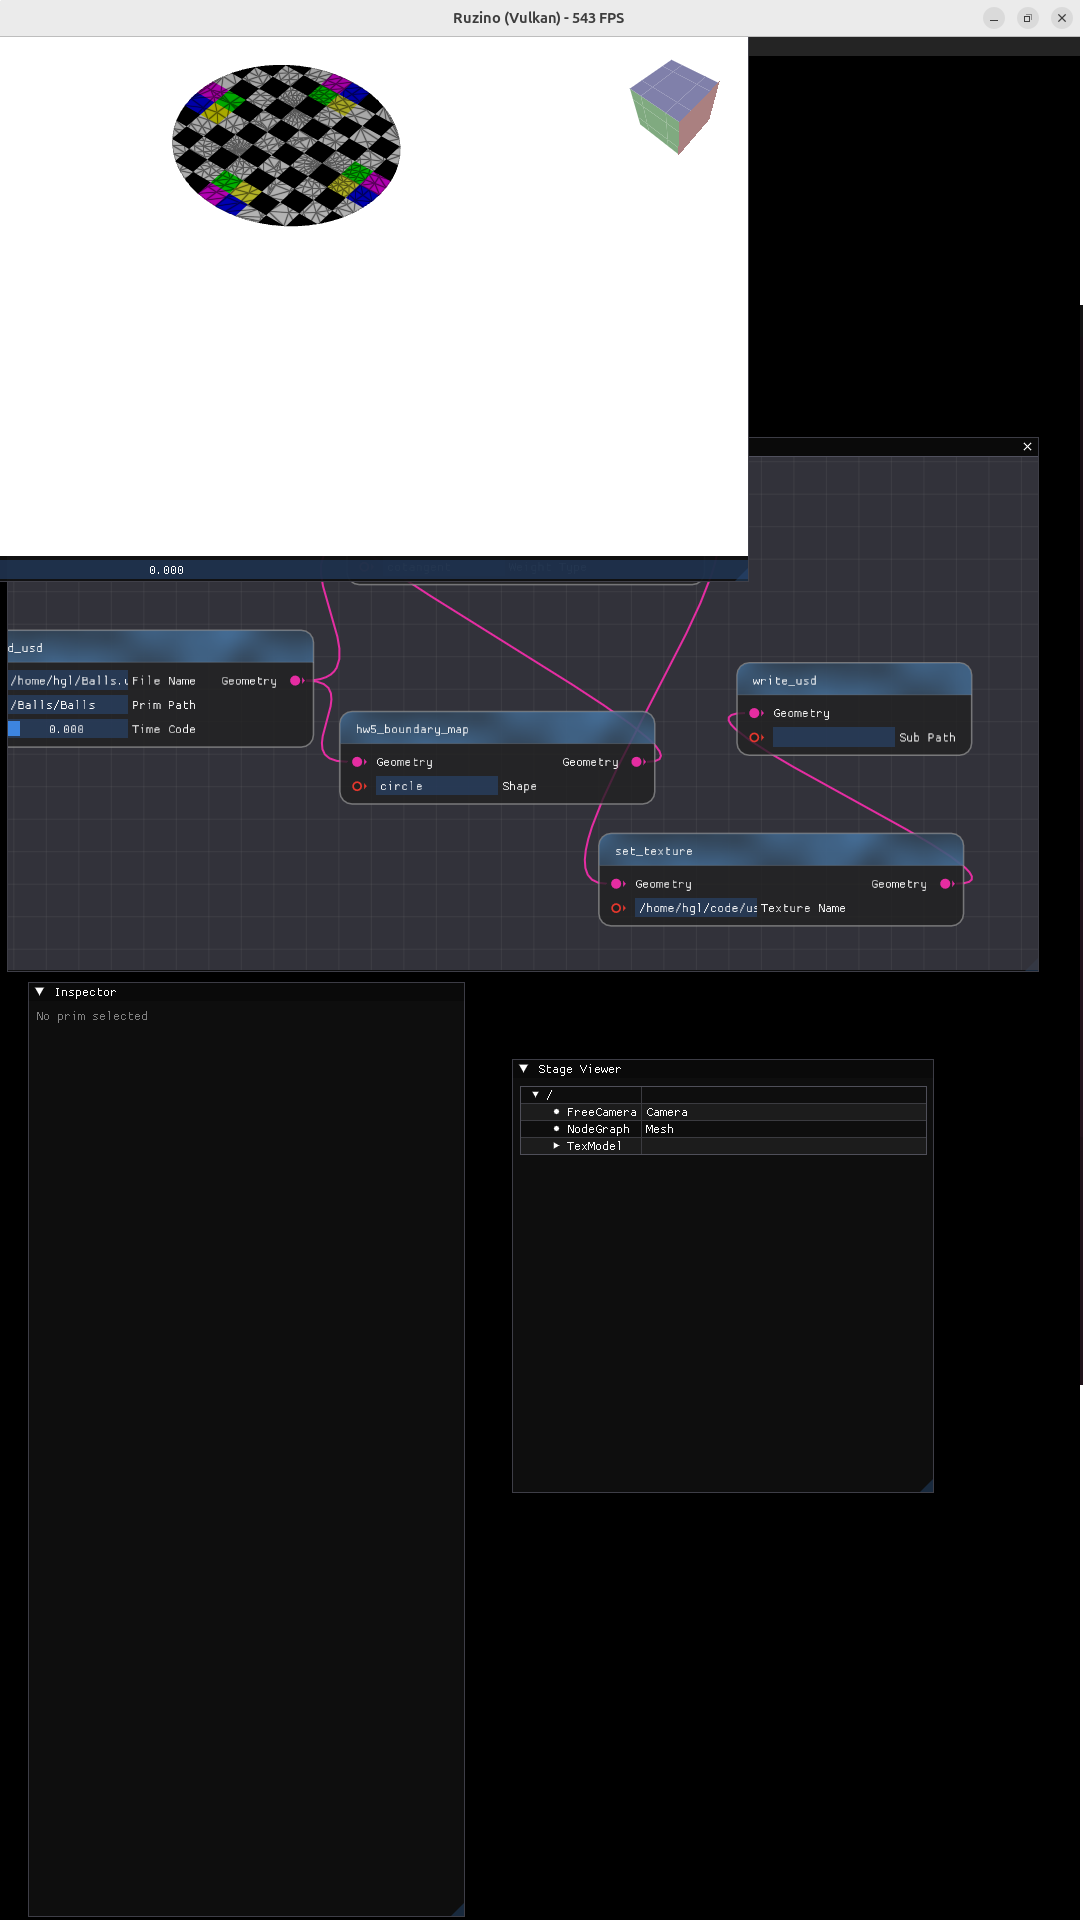
\includegraphics[width=0.6\textwidth]{pictures/贴图.png}
  \caption{将参数化回写至立体并贴上 \texttt{test.png} 的效果（2D UV 在立体表面上的展示）}
\end{figure}

\begin{figure}[H]
  \centering
  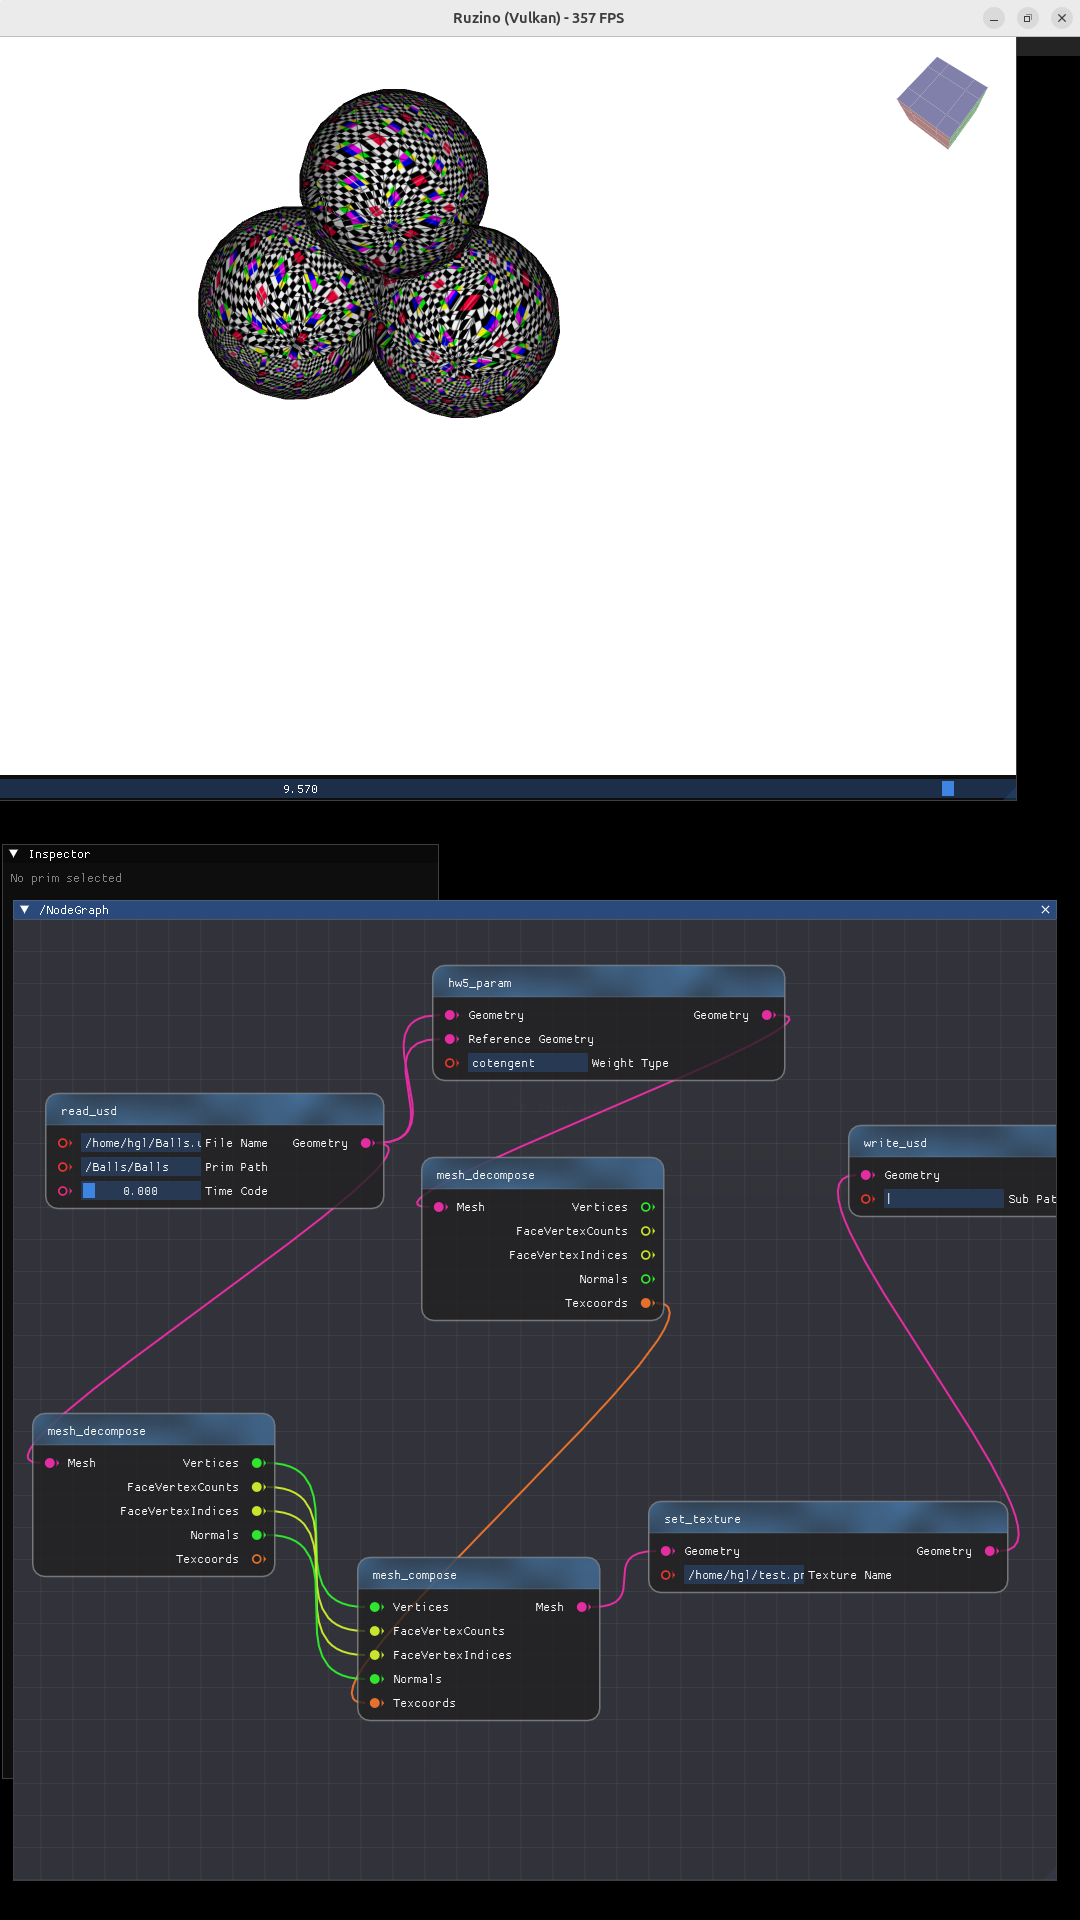
\includegraphics[width=0.6\textwidth]{pictures/贴图_立体.png}
  \caption{贴图在立体视图下的最终效果（高分辨率视图）}
\end{figure}

\section{结果文件与提交说明}
- 已在本地生成并保存 USD：\verb|Homeworks/5_tutte_parametrzation/pdf/Results.usd|（请确认该文件在你打包提交时包含在压缩包中）。
- 提交包建议包含：修改过的节点源文件、\verb|report.pdf|（由本 \verb|report.tex| 编译）、\verb|stage.usdc| 或 \verb|Results.usd|、\verb|data/| 下的测试模型与纹理。

\section{讨论与结论}
- Uniform 权重结果简单稳定，但在纹理分布上通常会产生非均匀拉伸。Cotangent 权重考虑了原始几何角度，能在保形或减少局部失真方面更优。
- 将参数化 UV 回写到原始立体，并通过 \verb|set_texture| 赋材质，是验证参数化质量最直观的方法。
- 如需进一步量化，可计算拉伸度量或角度失真并绘制热图（可扩展为下一步工作）。



\end{document}
